\subsection{Método de Newton-Raphson}

El método de Newton-Raphson es un algoritmo iterativo para encontrar raíces de funciones reales. Utiliza la derivada de la función para aproximar la raíz a partir de un valor inicial \cite{newtons-method}. Según \cite{newton-optimization} el método de Newton es una de las herramientas fundamentales en análisis numérico, investigación de operaciones, optimización y control. Tiene numerosas aplicaciones en la ciencia de la administración, la investigación industrial y financiera, y la minería de datos.

\subsubsection{Fundamento teórico}

En el trabajo de \cite{Stewart2012_Una} se presenta la interpretación geométrica del método de Newton. Como se observa en la figura \ref{plot-newton-raphson}, $r$ representa la raíz que buscamos encontrar. El proceso comienza con una primera aproximación $x_1$, que puede obtenerse mediante suposición, a partir de un esbozo de la gráfica de $f$, o mediante un graficador. Se considera la recta tangente $L$ a la curva $y = f(x)$ en el punto $(x_1, f(x_1))$ y se determina su intersección con el eje $x$, la cual se etiqueta como $x_2$. La idea fundamental del método de Newton radica en que la recta tangente aproxima localmente a la curva, por lo que su intersección $x_2$ está próxima a la raíz $r$ buscada. Dado que la tangente es una recta, su intersección con el eje $x$ puede calcularse de manera directa.

\begin{figure}[h]
	\centering
	\shorthandoff{<>}
	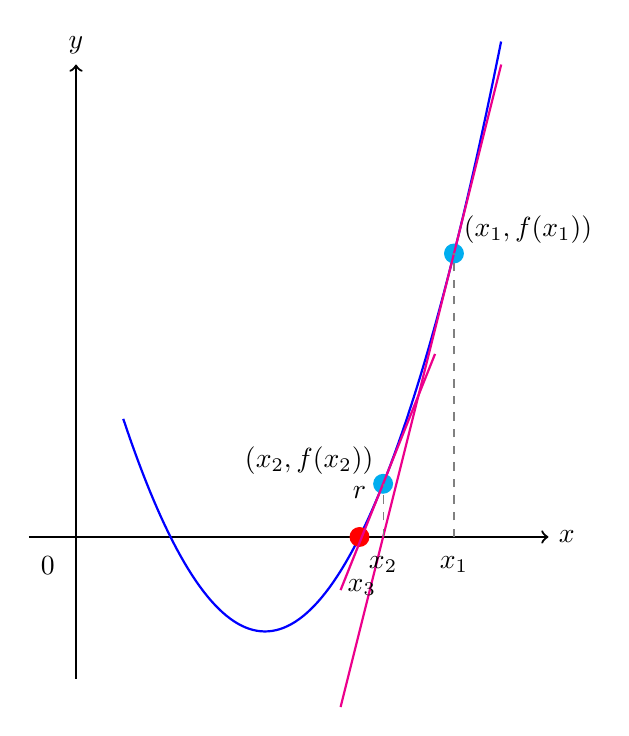
\begin{tikzpicture}[scale=1.2]
		% Axes
		\draw[->, thick] (-0.5,0) -- (5,0) node[right] {$x$};
		\draw[->, thick] (0,-1.5) -- (0,5) node[above] {$y$};
		\node at (-0.3,-0.3) {$0$};

		% Plot the function f(x) = (x-2)^2 - 1
		\draw[blue, thick, domain=0.5:4.5, samples=100] plot (\x, {(\x-2)^2 - 1});

		% Newton-Raphson iterations
		% For f(x) = (x-2)^2 - 1, f'(x) = 2(x-2)

		% Starting point x1
		\def\xone{4}
		\pgfmathsetmacro{\yone}{(\xone-2)^2 - 1}  % f(4) = 3
		\pgfmathsetmacro{\slopeone}{2*(\xone-2)}  % f'(4) = 4
		\pgfmathsetmacro{\xtwo}{\xone - \yone/\slopeone}  % x2 = 4 - 3/4 = 3.25

		% Second point x2
		\pgfmathsetmacro{\ytwo}{(\xtwo-2)^2 - 1}  % f(3.25)
		\pgfmathsetmacro{\slopetwo}{2*(\xtwo-2)}  % f'(3.25)
		\pgfmathsetmacro{\xthree}{\xtwo - \ytwo/\slopetwo}  % x3

		% Third iteration
		\pgfmathsetmacro{\ythree}{(\xthree-2)^2 - 1}
		\pgfmathsetmacro{\slopethree}{2*(\xthree-2)}
		\pgfmathsetmacro{\xfour}{\xthree - \ythree/\slopethree}  % x4

		% Root r (approximately at x=3, the right root)
		\def\xroot{3}
		\pgfmathsetmacro{\yroot}{(\xroot-2)*(\xroot-2) - 1}

		% Plot points on curve
		\fill[cyan] (\xone,\yone) circle (3pt);
		\fill[cyan] (\xtwo,\ytwo) circle (3pt);
		\fill[red] (\xroot,\yroot) circle (3pt);

		% Tangent lines (magenta) - properly calculated
		% Tangent at x1: y - f(x1) = f'(x1)(x - x1)
		% Rearranged: y = f'(x1)*x + (f(x1) - f'(x1)*x1)
		\draw[magenta, thick, domain=2.8:4.5] plot (\x, {\slopeone*(\x - \xone) + \yone});

		% Tangent at x2
		\draw[magenta, thick, domain=2.8:3.8] plot (\x, {\slopetwo*(\x - \xtwo) + \ytwo});

		% Vertical dashed lines
		\draw[gray, dashed] (\xone,0) -- (\xone,\yone);
		\draw[gray, dashed] (\xtwo,0) -- (\xtwo,\ytwo);

		% Labels for points
		\node[above right] at (\xone,\yone) {$(x_1, f(x_1))$};
		\node[above left] at (\xtwo,\ytwo) {$(x_2, f(x_2))$};
		\node[above] at (\xroot,0.3) {$r$};

		% Labels on x-axis (with adjusted positions to avoid overlap)
		\node[below] at (\xthree,-0.35) {$x_3$};
		\node[below] at (\xtwo,-0.1) {$x_2$};
		\node[below] at (\xone,-0.1) {$x_1$};

	\end{tikzpicture}
	\shorthandon{<>}
	\caption{Visualización del método de Newton-Raphson}
	\label{plot-newton-raphson}
\end{figure}

\subsubsection{Fórmula iterativa}

La fórmula de Newton-Raphson es:
\begin{equation}
	x_{n+1} = x_n - \frac{f(x_n)}{f'(x_n)}
\end{equation}

Geométricamente, esto representa extender la tangente a la curva en el punto $(x_n, f(x_n))$ hasta que intersecte el eje $x$.

\subsubsection{Algoritmo}

\begin{enumerate}
	\item Elegir un valor inicial $x_0$ cercano a la raíz esperada
	\item Calcular $f(x_n)$ y $f'(x_n)$
	\item Verificar que $f'(x_n) \neq 0$
	\item Calcular la siguiente aproximación: $x_{n+1} = x_n - \frac{f(x_n)}{f'(x_n)}$
	\item Verificar el criterio de convergencia: $|x_{n+1} - x_n| < \epsilon$ o $|f(x_{n+1})| < \epsilon$
	\item Si no se cumple el criterio, repetir desde el paso 2
\end{enumerate}


\subsection{Código matlab}

\begin{lstlisting}
format long;
syms x;
f_str = input('Ingrese la funcion para buscar una raiz: f(x) = ', 's');
f = str2sym(f_str);
a = input('Ingrese el valor inicial del intervalo: a = ');
b = input('Ingrese el valor final del intervalo: b = ');
if subs(f, x, a) * subs(f, x, b) > 0
    error('La funcion no corta el eje x en el intervalo dado.');
end
xn = (a + b) / 2;
errorEsperado = input('Ingrese el error requerido en decimales: E = ');
% Validacion de que la derivada no sea cero en el punto inicial
Df = diff(f, x);
if subs(Df, xn) == 0
    error('La derivada en el punto inicial es cero. El metodo de Newton puede no converger.');
end
% Imprimir encabezado de la tabla
fprintf('\n%s\n', repmat('=', 1, 90));
fprintf('%-10s %-20s %-20s %-20s %-20s\n', 'Iter (i)', 'Error Absoluto', 'Error (%)', 'Xn', 'Xn+1');
fprintf('%s\n', repmat('=', 1, 90));
fa = vpa(subs(f, x, xn));
fb = vpa(subs(Df, x, xn));
xn2 = xn - fa / fb;
Error = xn2 - xn;
% Calcular error porcentual para la primera iteracion
if xn2 ~= 0
    errorPorcentual = abs(Error / xn2) * 100;
else
    errorPorcentual = Inf;
end
% Imprimir primera iteracion
fprintf('%-10d %-20.10e %-20.10f %-20.10f %-20.10f\n', 1, abs(Error), errorPorcentual, double(xn), double(xn2));
xn = xn2;
i = 1;
while abs(Error) > errorEsperado
    fa = vpa(subs(f, x, xn));
    fb = vpa(subs(Df, x, xn));
    % Verificar que la derivada no sea cero antes de dividir
    if fb == 0
        error('La derivada es cero en la iteracion %d. El metodo no puede continuar.', i);
    end
    xn2 = xn - fa / fb;
    Error = xn2 - xn;
    
    % Calcular error porcentual
    if xn2 ~= 0
        errorPorcentual = abs(Error / xn2) * 100;
    else
        errorPorcentual = Inf;
    end
    
    i = i + 1;
    
    % Imprimir iteracion actual
    fprintf('%-10d %-20.10e %-20.10f %-20.10f %-20.10f\n', i, abs(Error), errorPorcentual, double(xn), double(xn2));
    
    xn = xn2;
end
% Linea de cierre de la tabla
fprintf('%s\n', repmat('=', 1, 90));
% Resultado final
fprintf('\nRaiz encontrada despues de %d iteraciones: %.10f\n', i, double(xn2));
fprintf('Error final: %.10e\n', abs(Error)); 
\end{lstlisting}
